\documentclass{beamer}
\usetheme{default}
\usepackage{graphicx}
\usepackage{hyperref}
\usepackage{amsmath,amssymb}
\usepackage{tikz}
\usetikzlibrary{arrows.meta, positioning}

\title{Hopfield Networks}
\author{}
\date{}

\begin{document}

% Slide 1: Title / Nobel Prize
\begin{frame}
\frametitle{2024 Nobel Prize in Physics}
\centering
\Large
Awarded to \textbf{John J.\ Hopfield} and \textbf{Geoffrey E.\ Hinton}\\[1em]
\normalsize
``for foundational discoveries and inventions that enable machine learning with artificial neural networks''\\[2em]
\small
October 8, 2024\\
Source: \url{https://www.nobelprize.org/prizes/physics/2024/press-release/}
\end{frame}

% Slide 2: Geoffrey Hinton bio
\begin{frame}
\frametitle{Geoffrey Hinton}
\begin{itemize}
    \item Nobel Prize in Physics 2024
    \item Born: 6 December 1947, London, United Kingdom
    \item Affiliation at the time of the award: University of Toronto, Toronto, Canada
    \item Prize share: 1/2
\end{itemize}
\vfill
\textbf{Work:} In 1983--1985, Geoffrey Hinton used tools from statistical physics to create the Boltzmann machine, which can learn to recognise characteristic elements in a set of data. The invention became significant, for example, for classifying and creating images.
\end{frame}

% Slide 3: Hopfield Network: Storing Memories
\begin{frame}
\frametitle{Hopfield Network: Storing Memories}
\begin{itemize}
    \item Can store memories as text/numbers
    \item Hard to retrieve
    \begin{itemize}
        \item Look through the entire library to find the right ``memory''?
    \end{itemize}
    \item The brain is not a library shelf
    \item Want something plausible
\end{itemize}
\end{frame}

% Slide 4: Hopfield Network
\begin{frame}
\frametitle{Hopfield Network}
\begin{itemize}
    \item The first attempt that kind of worked to model storing memories using networks
    \item Led to the development of the Boltzmann Machine -- a more advanced version of the Hopfield Network
    \item Boltzmann Machines were historically important in the development of modern neural networks
\end{itemize}
\end{frame}

% Slide 5: Hopfield Network structure + energy function
\begin{frame}
\frametitle{Hopfield Network Structure}
A Hopfield network is represented as a graph, with nodes taking values e.g.\ in $\{-1, 1\}$, and weighted edges representing the strength of the connections between the nodes.

\vspace{0.5em}
\begin{columns}[c]
\column{0.5\textwidth}
\centering
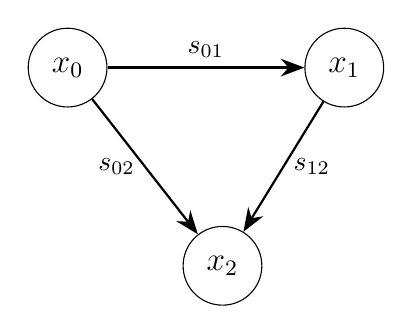
\begin{tikzpicture}[
    node distance=2.5cm,
    neuron/.style={circle, draw, minimum size=1cm, inner sep=0pt, font=\large},
    edge/.style={-{Stealth[length=3mm]}, thick}
]
    \node[neuron] (x0) {$x_0$};
    \node[neuron, right=of x0] (x1) {$x_1$};
    \node[neuron, below right=1.8cm and 1.25cm of x0] (x2) {$x_2$};

    \draw[edge] (x0) -- node[above] {$s_{01}$} (x1);
    \draw[edge] (x0) -- node[left] {$s_{02}$} (x2);
    \draw[edge] (x1) -- node[right] {$s_{12}$} (x2);
\end{tikzpicture}

\column{0.5\textwidth}
The ``memories'' of the Hopfield Network are the minima of the energy function $E$.

\vspace{1em}
Memories can be retrieved by finding the node values that minimize the energy function.
\[
E = -\sum_{i<j} x_i\, x_j\, s_{ij}
\]
\end{columns}
\end{frame}

% Slide 6: Example network with specific weights
\begin{frame}
\frametitle{Example: 3-Node Network}
For example, in the following network:

\vspace{0.5em}
\begin{columns}[c]
\column{0.45\textwidth}
\centering
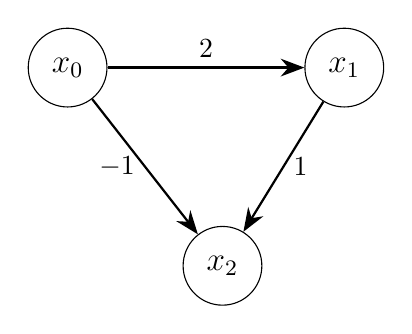
\begin{tikzpicture}[
    node distance=2.5cm,
    neuron/.style={circle, draw, minimum size=1cm, inner sep=0pt, font=\large},
    edge/.style={-{Stealth[length=3mm]}, thick}
]
    \node[neuron] (x0) {$x_0$};
    \node[neuron, right=of x0] (x1) {$x_1$};
    \node[neuron, below right=1.8cm and 1.25cm of x0] (x2) {$x_2$};

    \draw[edge] (x0) -- node[above] {$2$} (x1);
    \draw[edge] (x0) -- node[left] {$-1$} (x2);
    \draw[edge] (x1) -- node[right] {$1$} (x2);
\end{tikzpicture}

\column{0.55\textwidth}
\[
E = -(2x_0 x_1 - x_0 x_2 + x_1 x_2)
\]

\vspace{1em}
and the minima are:
\[
(-1,-1,-1),\; (-1,-1,1),
\]
\[
(1,1,-1),\; (1,1,1)
\]
\end{columns}
\end{frame}

% Slide 7: Storing and retrieving memories
\begin{frame}
\frametitle{Storing and Retrieving Memories}
\begin{itemize}
    \item \textbf{Retrieving memories:} find the minimum of the network
    \item \textbf{Storing memories:} adjust the weights a little so that there is a new minimum that corresponds to a memory; don't adjust the weights so much that there are ``spurious memories''
\end{itemize}
\end{frame}

% Slide 8: What are Hopfield Networks useful for? (Brain model)
\begin{frame}
\frametitle{What are Hopfield Networks useful for?}
\begin{itemize}
    \item A model for how the brain might store memories
\end{itemize}
\vfill
\centering
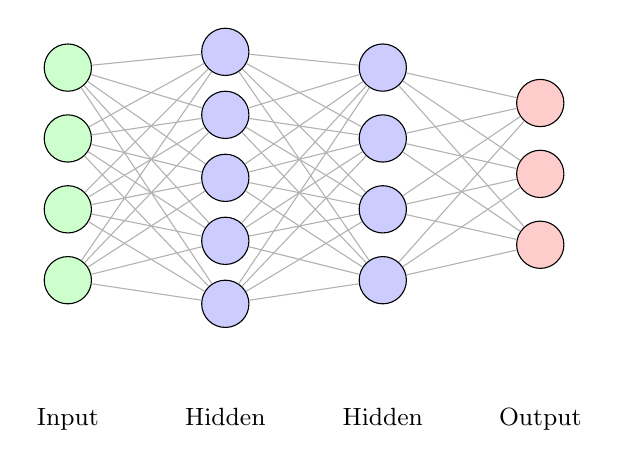
\begin{tikzpicture}[
    neuron/.style={circle, draw, fill=blue!20, minimum size=0.6cm, inner sep=0pt},
    input/.style={circle, draw, fill=green!20, minimum size=0.6cm, inner sep=0pt},
    output/.style={circle, draw, fill=red!20, minimum size=0.6cm, inner sep=0pt},
    conn/.style={-, thin, gray!60}
]
    % A simple neural network diagram as analogy
    % Input layer
    \foreach \i in {1,...,4} {
        \node[input] (I\i) at (0, -\i*0.9+2.7) {};
    }
    % Hidden layer 1
    \foreach \j in {1,...,5} {
        \node[neuron] (H\j) at (2, -\j*0.8+2.8) {};
    }
    % Hidden layer 2
    \foreach \k in {1,...,4} {
        \node[neuron] (G\k) at (4, -\k*0.9+2.7) {};
    }
    % Output layer
    \foreach \l in {1,...,3} {
        \node[output] (O\l) at (6, -\l*0.9+2.25) {};
    }
    % Connections
    \foreach \i in {1,...,4} {
        \foreach \j in {1,...,5} {
            \draw[conn] (I\i) -- (H\j);
        }
    }
    \foreach \j in {1,...,5} {
        \foreach \k in {1,...,4} {
            \draw[conn] (H\j) -- (G\k);
        }
    }
    \foreach \k in {1,...,4} {
        \foreach \l in {1,...,3} {
            \draw[conn] (G\k) -- (O\l);
        }
    }
    \node[below=0.3cm] at (0, -2.1) {\small Input};
    \node[below=0.3cm] at (2, -2.1) {\small Hidden};
    \node[below=0.3cm] at (4, -2.1) {\small Hidden};
    \node[below=0.3cm] at (6, -2.1) {\small Output};
\end{tikzpicture}

\vspace{0.5em}
\small Biological neurons connect to each other, forming networks. Hopfield Networks model this with weighted connections between nodes.
\end{frame}

% Slide 9: What are Hopfield Networks useful for? (Retrieving)
\begin{frame}
\frametitle{What are Hopfield Networks useful for?}
\begin{itemize}
    \item Retrieving things that look \emph{like} memories
    \begin{itemize}
        \item Store enough memories of faces
        \item Now find minima: they are either real memories or they look \emph{like} memories
    \end{itemize}
\end{itemize}
\end{frame}

% Slide 10: What are Hopfield Networks useful for? (Outlier detection)
\begin{frame}
\frametitle{What are Hopfield Networks useful for?}
\begin{itemize}
    \item Outlier detection
    \item New data point: does it look like previous memories?
    \begin{itemize}
        \item If energy high: no, might be fake
        \item If energy low: probably real (or a good fake)
    \end{itemize}
\end{itemize}
\end{frame}

\end{document}
